%% This is file `sample-authordraft.tex',
%% generated with the docstrip utility.
%%
%% The original source files were:
%%
%% samples.dtx  (with options: `authordraft')
%% 
%% IMPORTANT NOTICE:
%% 
%% For the copyright see the source file.
%% 
%% Any modified versions of this file must be renamed
%% with new filenames distinct from sample-authordraft.tex.
%% 
%% For distribution of the original source see the terms
%% for copying and modification in the file samples.dtx.
%% 
%% This generated file may be distributed as long as the
%% original source files, as listed above, are part of the
%% same distribution. (The sources need not necessarily be
%% in the same archive or directory.)
%%
%% The first command in your LaTeX source must be the \documentclass command.
\documentclass[sigconf]{acmart}
%% NOTE that a single column version may be required for 
%% submission and peer review. This can be done by changing
%% the \doucmentclass[...]{acmart} in this template to 
%% \documentclass[manuscript,screen,review]{acmart}
%% 
%% To ensure 100% compatibility, please check the white list of
%% approved LaTeX packages to be used with the Master Article Template at
%% https://www.acm.org/publications/taps/whitelist-of-latex-packages 
%% before creating your document. The white list page provides 
%% information on how to submit additional LaTeX packages for 
%% review and adoption.
%% Fonts used in the template cannot be substituted; margin 
%% adjustments are not allowed.
%%
%% \BibTeX command to typeset BibTeX logo in the docs
\AtBeginDocument{%
  \providecommand\BibTeX{{%
    \normalfont B\kern-0.5em{\scshape i\kern-0.25em b}\kern-0.8em\TeX}}}

%% Rights management information.  This information is sent to you
%% when you complete the rights form.  These commands have SAMPLE
%% values in them; it is your responsibility as an author to replace
%% the commands and values with those provided to you when you
%% complete the rights form.


\setcopyright{none}
\copyrightyear{2021}
\acmYear{2021}


%% These commands are for a PROCEEDINGS abstract or paper.
\acmConference[Seminar Data Science]{Ulm: Seminar Data-Science}{20/21}{Ulm, Germany}
\acmBooktitle{University Ulm: Seminar Data Science}

%%
%% Submission ID.
%% Use this when submitting an article to a sponsored event. You'll
%% receive a unique submission ID from the organizers
%% of the event, and this ID should be used as the parameter to this command.
%%\acmSubmissionID{123-A56-BU3}

%%
%% The majority of ACM publications use numbered citations and
%% references.  The command \citestyle{authoryear} switches to the
%% "author year" style.
%%
%% If you are preparing content for an event
%% sponsored by ACM SIGGRAPH, you must use the "author year" style of
%% citations and references.
%% Uncommenting
%% the next command will enable that style.
%%\citestyle{acmauthoryear}
\usepackage{tikz}
\usepackage{amsmath}
\DeclareMathOperator*{\argmax}{arg\,max}
\DeclareMathOperator*{\argmin}{arg\,min}
%%
%% end of the preamble, start of the body of the document source.
\begin{document}

%%
%% The "title" command has an optional parameter,
%% allowing the author to define a "short title" to be used in page headers.
\title{Temporal Graph Embedding}

%%
%% The "author" command and its associated commands are used to define
%% the authors and their affiliations.
%% Of note is the shared affiliation of the first two authors, and the
%% "authornote" and "authornotemark" commands
%% used to denote shared contribution to the research.
\author{Justin Mücke}
\email{justin.muecke@uni-ulm.com}
\affiliation{%
  \institution{University Ulm}
  \streetaddress{Albert-Einstein-Allee}
  \city{Ulm}
  \country{Germany}
  \postcode{89077}
}



%%
%% By default, the full list of authors will be used in the page
%% headers. Often, this list is too long, and will overlap
%% other information printed in the page headers. This command allows
%% the author to define a more concise list
%% of authors' names for this purpose.
\renewcommand{\shortauthors}{Justin Mücke}

%%
%% The abstract is a short summary of the work to be presented in the
%% article.
\begin{abstract}
 Temporal graph embedding is the process of transforming a graph, which changes over time, into a set of vectors. 
 To show how this is done, this paper goes over different methods to use on static graphs like DeepWalk and node2vec, and show how these can be modified to be applied on temporal ones as well. 
 The different methods were chosen depending on how well they help to show different aspects of the field.
 Furthermore, there will be different real world applications discussed.
\end{abstract}


%%
%% Keywords. The author(s) should pick words that accurately describe
%% the work being presented. Separate the keywords with commas.
\keywords{Temporal Graph, Embedding}

%% A "teaser" image appears between the author and affiliation
%% information and the body of the document, and typically spans the
%% page.


%%
%% This command processes the author and affiliation and title
%% information and builds the first part of the formatted document.
\maketitle

\section{Introduction}
With the surge of Facebook, Twitter and Instagram, huge and quickly changing social networks became a part of the everyday life of most people.
Until recent, a lot of real life networks were only representable as static graphs. If it was necessary to look at the development of a network, the only way was to use a set of static graphs and analyze them one by one.
Out of the inconvenience of this procedure the use of temporal graphs was proposed. These capture the whole evolution of a network in one construct, making it easier to work with them.
%% EMBEDDING
To make the analyzation viable, graphs get embedded into sets of vectors, to act as an accurate representation. 
%% APPLICATIONS
These vectors can be used to perform a variety of tasks, e.g. comparing two networks with each other.
%% GOAL 
The goal of this paper is to give an overview, which methods were used to analyze static graphs, and to show examples of how these were modified to work on 
temporal graphs.
%% SECTIONS
In the second section will be the fundamental knowledge. The third section will tackle the problem of static graph embedding before the fourth section will show how to
use them in a temporal context. Lastly, there will be a few examples of real world usage. 


\section{Preliminary}
To start this paper out, let's first create a level playing field for all readers by laying out what exactly a Graph is, 
how it can change over time and what is meant when talking about embedding.



\subsection{Graphs}
A graph is a mathematical construct which is used in a variety of tasks. It is often used to model relationships between 
entities, thus making it possible to operate on such structures to, for example, analyze them.\\
Mathematically it is consisting of two sets \(G = (V, E)\), where V consists of all the vertices of the Graph, and E of all the edges, represented through a tuple of two vertices.
To visualize graphs its common practice to denote nodes as circles with connections between them as edges as seen in figure 1.

 \begin{figure}[h]
  \begin{center}
    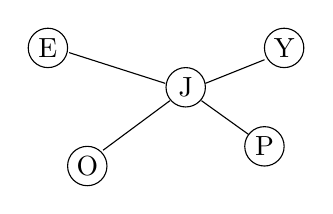
\begin{tikzpicture}
      \draw (0,-0.5) node [circle,inner sep=0pt,draw,minimum size=0.5cm] {E};
      \draw (1.75,-1) node [circle,inner sep=0pt,draw, minimum size=0.5cm] {J};
      \draw (0.5,-2) node [circle,inner sep=0pt,draw, minimum size=0.5cm] {O};
      \draw (3,-0.5) node [circle,inner sep=0pt,draw, minimum size=0.5cm] {Y};
      \draw (2.75,-1.75) node [circle,inner sep=0pt,draw, minimum size=0.5cm] {P};

      \draw (0.27, -0.56) -- (1.49, -0.95);
      \draw (1.55, -1.17) -- (0.7, -1.8);
      \draw (2, -0.95) -- (2.75, -0.65);
      \draw (1.95, -1.17) -- (2.55, -1.6);
    \end{tikzpicture}
\end{center}
\caption{Graph described through \\ \( G = (\{E,O,Y,P,J\}, \{(J,E),(J,O), (J,P), (J,Y)\}) \).}
\end{figure}

\subsection{Temporal Graphs}
A temporal graph, on the other hand, is a graph that changes its structure over time. A structural change is defined as the replacement of object in \(V\) or \(E\).
The graph \(G\) is then represented through \(G = (V,E)\) where \(V_T\) contains every vertex and \(E_T\) every node, that is in the graph at one point.
The Evolution of the graph is defined as \(G_{E_T} = \{G_1, \ldots, G_T\}\). Here \(G_i\) is the static graph after time \(i*\Delta t\).
\cite{DBLP:journals/corr/abs-1905-05304}

\subsection{SkipGram}
SkipGrams are a form of neural networks that are used heavily in the natural language processing. It is used to find the context of words in a training document.
This network gets trained by having a document as input and learning which words are in a fixed distance to each other \cite{Rong.11.11.2014}.
It consists of one input-, one hidden- and one output layer. 
Each word in our text is assigned an ID through a one-hot coded vector, so that each word \(w_i\) can be represented like \((0_1, 0_2, \ldots, 0_{i-1}, 1_i, 0_{i+1}, \ldots 0_n)\).
It then computes how likely it is for each word to be the neighbor of each other word and transforms it into a distribution using a softmax-function \cite{gao2018properties}.



\section{Static embedding}
Embedding is a process in which the graph \(G = (V_g, E_g)\) is transformed into a set of vectors \(V\).
These capture the graph topology, vertex-to-vertex relationship as well as other relevant information.
This way, it is more accessible for analyzing the graph and comparing it to others.
Overall we can divide graph embedding techniques into two categories; 
vertex embedding and graph embedding. \\
When using vertex embedding, there has to be one vector \(v\) for each node in \(G\), so that \(|V| = |V_g|\). This is used to make prediction 
on a node level.\\
When using graph embedding, there is one vector representing the whole graph. This method is most useful to analyze the data on a graph level e.g.
comparing two graph structures with each other.\\
In order to achieve this transformation there are several methods available.

\subsection{Word2Vec}
The first method is word2vec which is the foundation for many other methods. 
It takes a text \(T = (w_1, w_2, \ldots, w_n)\) as input and, using SkipGram networks, returns a set of vectors \(V\), where \(v_i\) is a distribution describing how likely it is for each word 
to be a direct neighbor to a root word. The neighbors of a word \(w_c\) are defined as \(\{w_i | i \in (c-\epsilon, c+\epsilon)\}\) where \(\epsilon\) describes a predefined window size as seen in figure 2.
With this, the whole text is represented solely through vectors, where similar words have similar vectors.
One way to achieve this, is to train a SkipGram neural network to create the distributions. 
\begin{figure}[h]
  \begin{center}
    \scalebox{0.8}{
    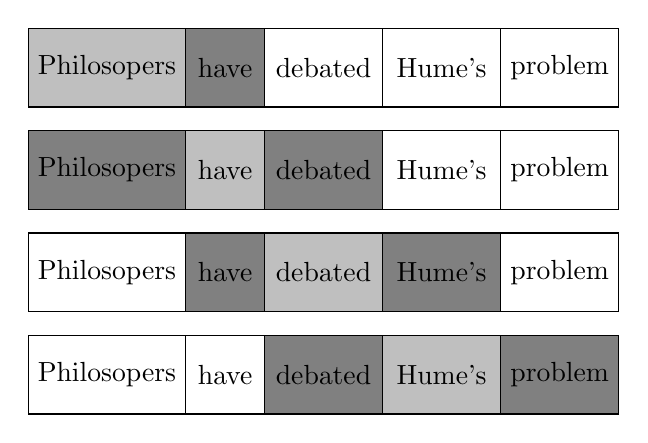
\begin{tikzpicture}
      \draw (0,0) rectangle (2,1) node[pos=.5] {Philosopers};  
      \draw (2,0) rectangle (3,1) node[pos=.5] {have};  
      \draw [fill=gray](3,0) rectangle (4.5,1) node[pos=.5] {debated};  
      \draw [fill=lightgray](4.5,0) rectangle (6,1) node[pos=.5] {Hume's};  
      \draw [fill=gray](6,0) rectangle (7.5,1) node[pos=.5] {problem}; 

      \draw (0,1.3) rectangle (2,2.3) node[pos=.5] {Philosopers};  
      \draw [fill=gray](2,1.3) rectangle (3,2.3) node[pos=.5] {have};  
      \draw [fill=lightgray](3,1.3) rectangle (4.5,2.3) node[pos=.5] {debated};  
      \draw [fill=gray](4.5,1.3) rectangle (6,2.3) node[pos=.5] {Hume's};  
      \draw (6,1.3) rectangle (7.5,2.3) node[pos=.5] {problem}; 

      \draw [fill=gray](0,2.6) rectangle (2,3.6) node[pos=.5] {Philosopers};  
      \draw [fill=lightgray](2,2.6) rectangle (3,3.6) node[pos=.5] {have};  
      \draw [fill=gray](3,2.6) rectangle (4.5,3.6) node[pos=.5] {debated};  
      \draw (4.5,2.6) rectangle (6,3.6) node[pos=.5] {Hume's};  
      \draw (6,2.6) rectangle (7.5,3.6) node[pos=.5] {problem}; 

      \draw [fill=lightgray](0,3.9) rectangle (2,4.9) node[pos=.5] {Philosopers};  
      \draw [fill=gray](2,3.9) rectangle (3,4.9) node[pos=.5] {have};  
      \draw (3,3.9) rectangle (4.5,4.9) node[pos=.5] {debated};  
      \draw (4.5,3.9) rectangle (6,4.9) node[pos=.5] {Hume's};  
      \draw (6,3.9) rectangle (7.5,4.9) node[pos=.5] {problem}; 

    \end{tikzpicture}}
  \end{center}
  \caption{Light-gray word, with dark-gray neighbor and \(\epsilon = 1\).}
\end{figure}
\cite{Godec.31.12.2018}


\subsection{DeepWalk}
This method is a continuation of the word2vec approach, but now the input is not a text, but a graph \(G = (V,E)\)
It consists of three steps. The first being the sampling, where random walks are performed from each node.
Hereby, a random walk is a path in the graph from a starting point \(v_i\) of defined length \(\lambda\). 
The following nodes are generated by: 
\begin{center}
  \(P(v_i = x|v_{i-1} = y) = \begin{cases} \frac{\pi_{xy}}{Z} &\text{if} (x,y) \in E \\ 0 & \text{otherwise} \end{cases}\)
\end{center} 
where \(\pi_{xy}\) is the probability between nodes \(x\) and \(y\) with \(Z\) as the normalizing constant.\\
It is sufficient to perform \(32-64\) random walks per Node. The resulting paths are of the same structure as sentences in a text, so 
the word2vec method can now be used on it.
The result is a set of vectors \(V\) where each vector \(v_i\) is a distribution of the probability that two nodes are next to each other.
\cite{Godec.31.12.2018}


\subsection{Node2Vec}
This is an optimized version of DeepWalk.
Again, there is the sampling phase in the beginning. The difference in the methods is, that in node2vec the random walks are now biased and not completely random.
An order for the random walk is defined through two parameters \(p\) and \(q\). To evaluate which node to visit next the walk looks at the transition probability
\(\pi_{xy}\) on the edge \((x,y)\). This probability is now defined as \(\pi_{xy} = \alpha_{pq}(x, y) \cdot w_{xy}\) where \(w_{xy}\) is the weight assigned to the edge \((x,y)\) and:
\begin{center}
 \(\alpha_{pq}(xy) = \begin{cases} \frac{1}{p} & \text{if } d_{xy} = 0 \\ 1 & \text{if } d_{xy} = 1 \\\frac{1}{q} & \text{if } d_{xy} = 2 \\\end{cases}\)
\end{center}
with \(d_{xy}\) being the shortest path between nodes \(x\) and \(y\).
Hereby, our parameter \(p\) defines how likely it is to revisit a node of the walk. Setting \(p\) to a higher value encourages the walk to go deeper into the graph, whereas a small value 
ensures the walk to stay local around the starting point. 
In contrast, \(q\) describes the preference of nearer or further nodes. For \(q>1\) the walk favors closer nodes, for \(q<1\) nodes that are further away.
\cite{Grover.03.07.2016}

\subsection{Structural Deep Network Embedding}
In contrast to the methods used before, SDNE does not use random walks. It aims to preserve local pairwise similarity which characterizes the local structure, and 
as well as the global network structure.
To achieve this, two autoencoder neural networks are used. These get an adjacency vector as input and construct node adjacency vectors as output.
Then the distance between the two outputs is computed and added to the loss function of the network.
The total loss function is then calculated through summation of the distance loss plus the losses of the two encoders.
At the end remains a collection of adjacency vectors which describe the graph structure.
\cite{Godec.31.12.2018}


\subsection{Graph2Vec}
Now not the nodes are represented by vectors, but the whole graph. For that, there are once again three steps. 
In the first step the algorithm creates sub-graphs for each node and encodes them once again in a one-hot code. We then use these sub-graphs to train the network used in 
word2vec to maximize the probability that a predicted sup-graph exists in the input graph. The embedding is then the result of the network.
\cite{Godec.31.12.2018}



\section{Embedding of Temporal Graphs}
Let \(G = (V,E)\) be a temporal graph with \(G_{E_T} = \{G_1, \ldots, G_T\}\) as its evolution over the time steps \(T\).
The goal is now, to create a vector space which can be used to analyze the graph to find anomalies in it, compare it to other graphs, classify nodes or predict if 
certain links are going to exist.
Depending on which outcome is wanted, different methods have to be used to optimize it. For predictions on the node level like node classification and link prediction a node-level algorithm should be used. 
On the other hand, a graph-level algorithm should be used to compare graphs with each other and to find anomalies, as shown in 3.3.

\subsection{tNodeEmbed}
As aforementioned, a node-level algorithm should be used to perform e.g. link predictions and node classification. 
One proposed algorithm of that form is \emph{tNodeEmbed}. Here, the embedding can be split into three parts: 
%% Work up: initialisierung -> auslenkung -> zusammenfassung
\subsubsection{Initialization}
To start out, the algorithm initializes a representative vector \(Q_t \in \mathbb{R}^{T \times d}\) for each node \(v\) in all graphs \(G_{t_1}, \ldots, G_{t_T} \), where \(d\) is the embedding size, and \(T\) the number of time steps.
These vectors are created using the node2vec algorithm discussed in 2.3.3.

\subsubsection{Node alignment}
A downside to node2vec is that, when running on a graph, it aims to minimize the word embedding distances but not consistency over multiple trainings.
The resulting embedding could be in a two-dimensional space for example. It lays in a x-y-plane. Now imagine a rotation around the unused z-axis. The resulting graphs have the
same structure but different orientation in the plane, thus not having an alignment, as seen in figure 3.
Similarly, when embedding two graphs \(G_{t_i}\) and \(G_{t_j}\) it is not guaranteed that, even if the graphs are identical, their axes align.
To adjust those embeddings, tNodeEmbed uses an orthogonal transformation between embeddings at two time points \(t_i\) and \(t_j\)\cite{Schonemann.1966}.
Used in this algorithm, it takes the matrix \(Q_t \in \mathbb{R}^{d\times |V|}\) of node embeddings at time \(t\). Then the matrices get aligned iteratively starting from the earliest time step.
For the alignment an orthogonal matrix \(R\) between \(Q_t\) and \(Q_{t+1}\) is needed to result in the final embedding \(Q'_t = RQ_t\).
The matrix is approximated by : 
\begin{center}
  \(R_{t+1} = \argmin\limits_{R s.t. R^TR =I} \|RQ_{t+1} - Q_t\| \)
\end{center}
where \(R_{t+1} \in \mathbb{R}^{d \times d} \) is the transformation which fits the time steps the most.
\begin{figure}[h]
  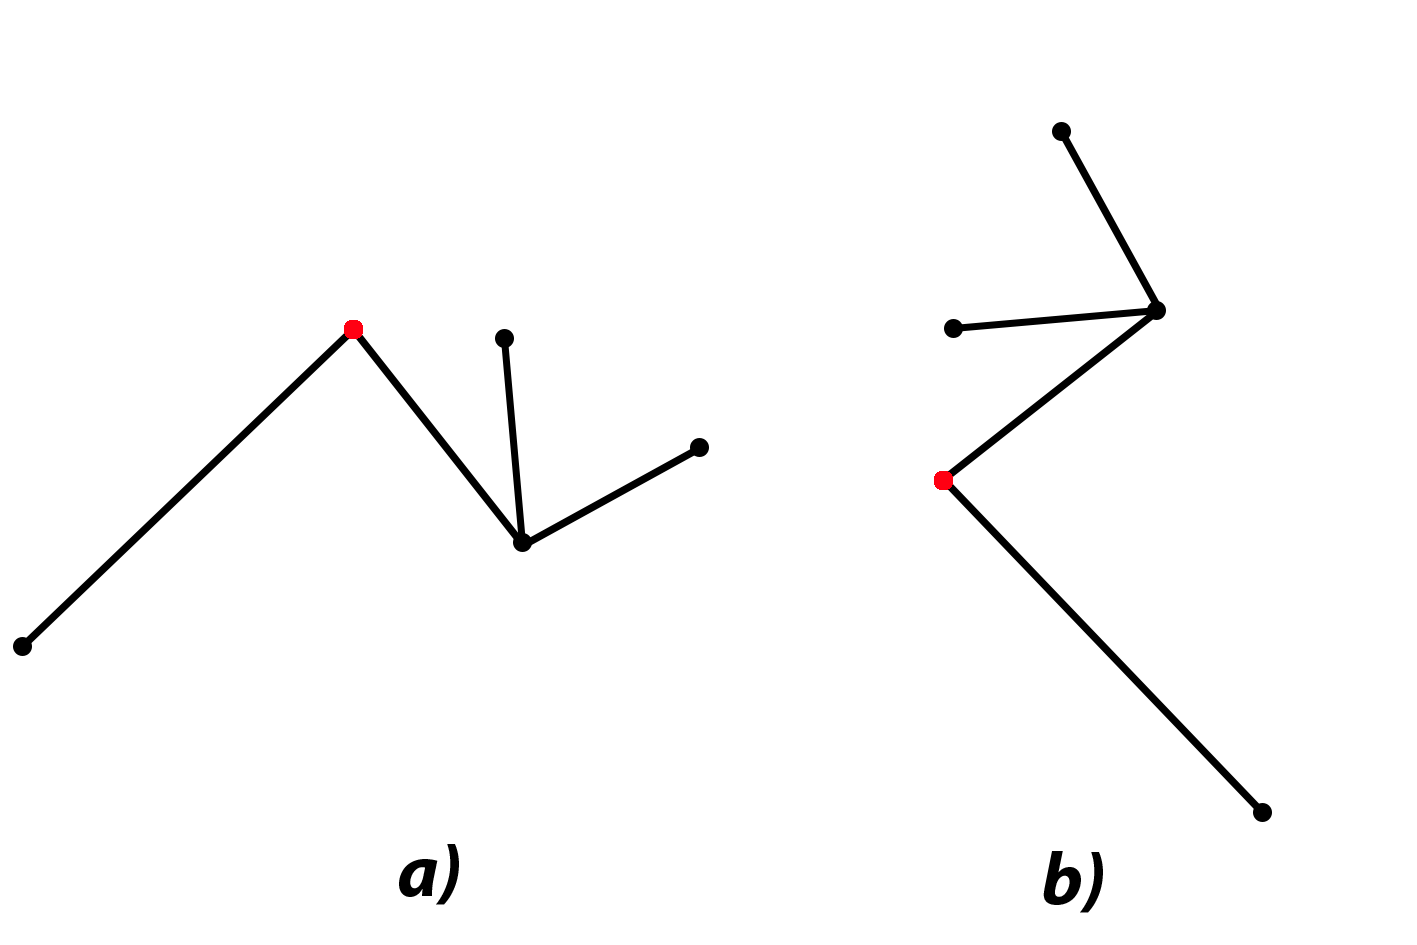
\includegraphics[scale=0.1]{UnalignedGraphs.png}
  \caption{a) embedding of the first graph. b) embedding of the second graph. The red node do not align even though the graph structure is the same.}
\end{figure}

\subsubsection{Finalization}
The algorithm works in such a way, that the only difference in the algorithm, between the two outcomes, is the loss function. 
For the node classification task it uses a categorical cross-entropy loss:
\begin{center}
 \(L_{task} = -\sum\limits_{v\in V} \log {Pr(class(v)|f_T(v))}\)
\end{center}
For the link prediction task it considers a binary classification loss: 
\begin{center}
  \(L_{task} = -\sum\limits_{v_1, v_2 \in V} \log{Pr((v_1,v_2)\in E | g(f_T(v_1), f_T(v_2)))}\)
\end{center}
The Algorithm now wants to learn a function \(F_T\) so that \(f_T(v) = F_T(v,G_1, \ldots, G_T)\) that optimizes for \(L_{Task}\).
The function is defined recursively as: 
\begin{center}
  \(f_{t+1} = \sigma(Af_t(v) + BQ_tR_tv)\) \\
  and \(f_0(v) = \vec{0}\)
\end{center}
with \(A,B,R_t\) and \(Q_t\) being matrices, \(v\) again being a one-hot vector representing a node and \(\sigma\) being an activation function.
The final temporal embedding is now defined as the minimization of the loss-function:
\begin{center}
  \( L = \min\limits_{A,B,Q_1, \ldots Q_T,R2, \ldots, RT} L_{task}\).
\end{center}
Now, it is only a Question on how to define \(A,B\) and \(\sigma\).
Due to the steps beforehand, each node is associated with a matrix \(X^{(v)} \in \mathbb{R}^{T \times d}\) consisting of 
all embeddings \(T\), which are of size\(d\), thus the whole graph can be seen as \(G_X = X^{(v_1)},\ldots, X^{(v_{|V|})}\).
To perform the wanted graph-prediction tasks, the matrices representing each node now need to be reduced into a single vector, so it can be used as input for a classifier, as in the static embeddings.
For this it is proposed to use recurrent neural networks with long short term memory. These calculations come with a high computational cost.
\cite{Singer.2019}

\subsection{tdGraphEmbed}
The goal of this algorithm is to create a mapping function that embeds a graph \(G_t\) into a \(d-\)dimensional space \(\mathbb{R}^d\) with \(d \in \mathbb{Z}\).
This embedding captures not only the nodes' evolution over time, but also the graphs structure. Additionally, graphs with a similar structure have an embedding close to each other.
To achieve this, the algorithm follows these steps:
\subsubsection{Random Walks}
The algorithm uses random walks \(W\), as described in 2.3.2, to sample the graphs. Using these random walks, the algorithm estimates the likelihood of the graph
at time \(t\) being completely described through them. This likelihood is defined as:
\begin{center}
  \(Pr(G_t|W_{v_1}, W_{v_2},\ldots, W_{v_k}))\)
\end{center}
with \(v_1, v_2, \ldots, v_k \ in V_t\).
Such random walks are initiated \(\gamma\) times for each node in \(V_t \in G_t\).
Those random walks are then concatenated forming a document describing the graph.
\subsubsection{Context Nodes}
After all the documents are formed, the algorithm predicts the next node in a random walk. 
The nodes in a neighborhood, later referred to as context nodes, are defined as: 
\begin{center}
  \(N_s(v_i^t)=\{v_{i-\omega}^t, \ldots, v_{i+\omega}^t\}\).
\end{center}
Using these and the graph \(G_t\) the algorithm maximizes the equation: 
\begin{center}
  \(\log{p(v_i^t | N_s(v_i^t), G_t)}\).
\end{center}
The goal is to learn a \(d-\)dimensional representation \(\phi\) where \(\phi(v_i^t)\) is the mapping of node
\(v_i \in V_t\) and \(\phi(G_t)\) the mapping of the graph. With this mapping and a soft-max function the equation above can be calculated with: 
\begin{center}
  \(p(V_i^t|N_s(v_i^t), G_t) = \frac{e^{\phi(v_i^t) \cdot h}}{\sum\limits_{j \in V_t} e^{\phi(v_j^t) \cdot h}}   \)\\
  where \(h=\sum\limits_{c \in N_s(v_i^t)} \phi(v_c^t) + \phi(G_t)\)
\end{center}
where \(G_t\) is the global context shared between all embeddings. This is combined with the local context of the Nodes.

\subsubsection{Optimization}
With these equations the output calculation for each random walk \(W\) can be simplified to: 
\begin{center}
  \(\max\limits_\phi \sum\limits_{t \in T}\sum\limits_{W\in G_t}\sum\limits_{v_i^t} -log\sum\limits_{j\in V_t} e^{\phi(v_j^t)\cdot h}\:\:\: +\phi(v_i^t \cdot h)\).
\end{center}
The calculating neural network is trained using gradient descent \cite{Ruder.15.09.2016}. For each step, a fixed-length context is sampled from a walk \(W\), with which the error gradient is calculated and used to update the parameters of the model.
The last equation also gets computationally expensive for large graphs, thus a negative sampling strategy is used \cite{Goldberg.15.02.2014}. To enhance the efficiency even more, 
the algorithm only considers nodes that are active in each time step instead of all nodes in \(V\). Active nodes are those, who change one or more property over a time step.
Even though, the optimizations influence the computation heavily, the embedding \(\phi\) is still accurate. \cite{Beladev.2020}


\section{Application}
Nowadays, graphs are used for a variety of applications. With it comes the need to analyze such graphs. They model e.g. Protein to Protein interactions in biology, social networks in social sciences and even  so-called word co-occurence in linguistics.
To understand and analyze those structures better, scientists have aimed to model such graphs and the interaction between different entities they contain.
Depending on the scientific task, it is either better to use a node-level or a graph-level algorithm\cite{Goyal.2018}.


\subsection{Node classification}
One application for node-level algorithms is \emph{node classification}. This is used when a lot of the information contained in graphs can be put into different categories e.g. gender, age, demographic and political beliefs. Those categories are called labels and can be applied to nodes in a graph representing e.g. users of a social network.
Such labels can then be used to recommend new connections between individuals, movies and music based on the interests and personalize advertisements.

\subsection{Link prediction}
Another use for node-level algorithms is link prediction, as it is looking at the relations between single nodes in the graph.
Every relation in a graph describing a social network, can be described  through an edge or link. So, whenever one entity engages another, the graph changes.
The link prediction problem defines the question, how likely it is, given a snapshot of such a social network, that members engage each other in the near future \cite{LibenNowell.op.2003}.
Everybody has an intuitive feeling for who would follow whom. Due to the fact that they may have the same friends, live in the same city or have the same hobbies. 
Link prediction is the attempt to make these intuitive thoughts more precise and have an underlying method on how to do so.

\subsection{Clustering}
With increasing graph size, increases the probability that two nodes share a lot of labels. 
Clustering aims to find such nodes and generate a sub-graph out of them. Using this, e.g. users of an online social network with the same interests can be quickly found as they are members of the same sub-graph.
It also enables to structure the network, as one can label whole sub-graphs instead of individual nodes \cite{Ding.2001}. Here as well, node-level algorithms are most likely used. 

\subsection{Similarity}
Another use for embeddings is answering the question of how alike two graphs are. For this purpose, a graph-level algorithm is optimal in contrast to the applications mentioned before. The more similar the topologies of the two graphs are, the closer the embeddings are to one another. This can be used on whole graphs or to see if a graph
contains multiple similar sub-graphs. If a sub-graph existed in another part of the graph, this information can be used to predict its evolution, as the earlier formed sub-graph can be used as reference point \cite{Beladev.2020}.

\subsection{Anomaly}
Using the evolution of temporal graphs, repeating trends can be found. With the repeating patterns it is also possible to find anomalies in the graph which do not adhere to the pattern.
This can be used to analyze how big of an impact e.g. political decisions can have on social constructs \cite{Beladev.2020}, or how active a community is. An example for the second one is 
the activity of the \emph{Game of Thrones} subreddit at the release of a new episode of the series, as seen in \cite{Beladev.2020}. 



\section{Conclusion}
Graph embedding techniques are effective methods of transforming graphs into a more suitable structure to analyze them. They enable a more convenient method to analyze the whole evolution of a graph.
Thanks to these embedding methods, tasks like clustering and link prediction are made possible.
In the last few years, the research in this area shifted towards the scalability of embedding methods to be able to work on graphs with millions of nodes \cite{Bruss.03.07.2019}.
A big problem with scalability right now is the high computation and space cost. Thus, a lot of research focuses on a way to make the expensive graph analytics more efficient \cite{Cai.22.09.2017}.


In my opinion, graph embedding in an essential and practical tool in the modern graph analysis. They help in various field, e.g. analyzing the effect of political decisions on social groups. %% Graphentheorie macht das -> Embedding hilft da
But also for the day-to-day life they have become very important. They can be used to recommend following new people on social media platforms like Instagram and Facebook, based on your hobbies and the people you are already following.
Furthermore, they can be used to find out what kind of music or movies you are interested in when using them on sites like Spotify and Netflix. 
With increasing scale of these algorithms, the insights they can give us on networks should become increasingly more precise. As I have high hopes for the developments of more efficient algorithms, I look forward to seeing what they can do in the future.


%% The next two lines define the bibliography style to be used, and
%% the bibliography file.
\bibliographystyle{IEEEtr}
\bibliography{citation}
%% If your work has an appendix, this is the place to put it.

\end{document}
%%
%% End of file `sample-authordraft.tex'.